\chapter{Metodologia}
\label{chap:Metodologia}

\section{Preparação do Estudo de caso}
\label{chap:Preparação}
Nesse estudo de caso vai ser utilizado uma ferramentas BPMS para ser feito os testes junto com um processo criado para o estudo de caso. A ferramenta que será utilizada é o Bizagi. Essas ferramenta foi escolhida pelo motivo de ser uma ferramenta de fácil uso e a sua curva de aprendizado é menor se comparado a outros BPMS.



\section{Processo BPM Utilizado}
\label{chap:Processo-Utilizado}
Para inicio do estudo de caso, será feito um processo chamado Avaliação do Desenvolvedor. Onde nesse processo é implementado como parte de uma estratégia de melhoria contínua. O objetivo é avaliar o desempenho de cada desenvolvedor de acordo com a competência requisitos, e promover o seu desenvolvimento profissional com valor feedback de desempenho.
 


Como se encontra na Figura abaixo e será modelado em ambas ferramentas, para que seja utilizado para os testes que serão feitos. 

\begin{figure}[h!]
	\centering
		\Caption{\label{fig:Avaliacao_do_Desenvolvedor} Avaliação do Desenvolvedor }	
		\UNIFORfig{}{
			\fbox{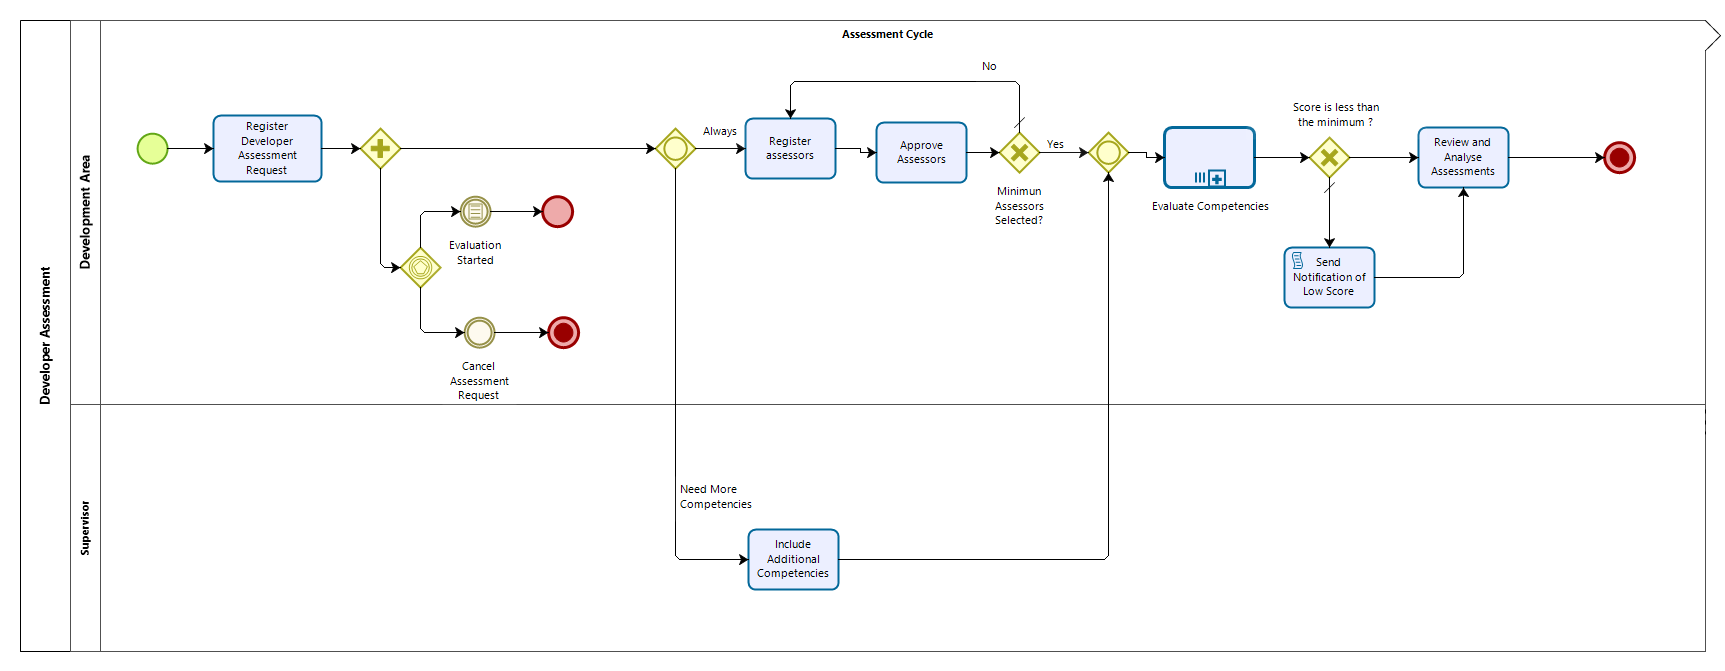
\includegraphics[width=15cm]{figuras/Developer_Assessment.png}}
		}
       	{
			\Fonte{Elaborado pelo autor}
		}	
	\end{figure}
    
Na figura abaixo temos o subprocesso Avaliação de Competência
\begin{figure}[h!]
	\centering
		\Caption{\label{fig:Avaliação de Competencia} Avaliação de Competência }	
		\UNIFORfig{}{
			\fbox{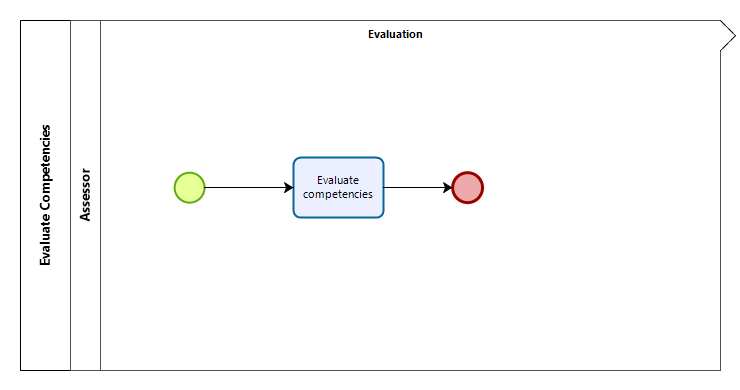
\includegraphics[width=15cm]{figuras/Evaluate_Competencies.png}}
		}
       	{
			\Fonte{Elaborado pelo autor}
		}	
	\end{figure}
    
\begin{figure}[h!]
	\centering
		\Caption{\label{fig:modelo_de_dados} Modelo de Dados }	
		\UNIFORfig{}{
			\fbox{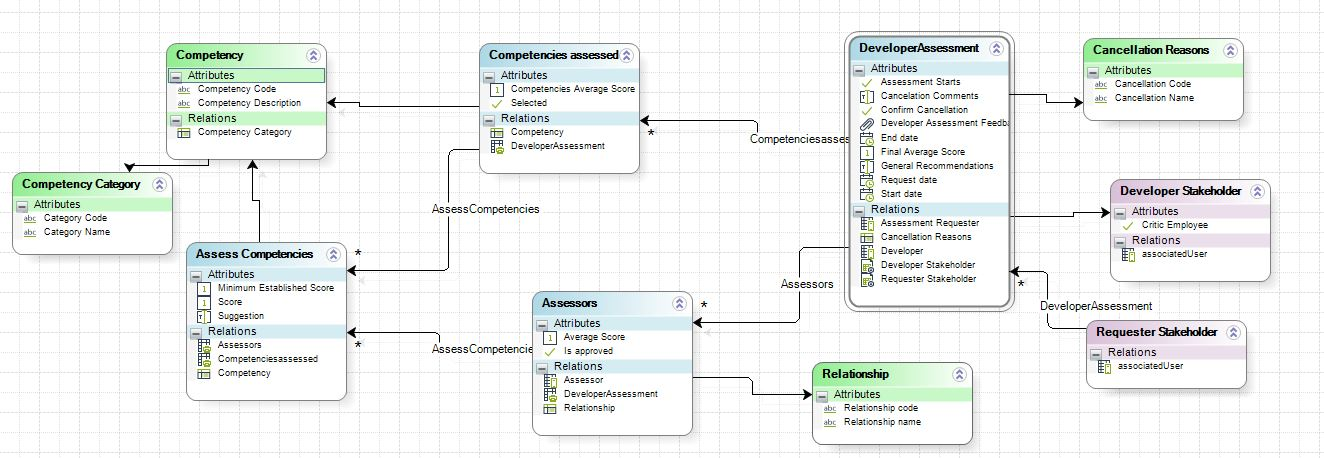
\includegraphics[width=15cm]{figuras/modelo_de_dados.JPG}}
		}
       	{
			\Fonte{Elaborado pelo autor}
		}	
	\end{figure}






%\section{Ferramentas BPMS}
%\label{chap:Ferramentas-BPMS}


%\subsection{Bizagi Studio}
%O Bizagi Studio é uma ferramenta \textit{freeware}, criada pela Bizagi, onde é reconhecida por ser  


%\section{Ferramentas de teste}
%\label{chap:Ferramentas-BPMS}

%será utilizado a ferramenta, chamada Selenium que é uma ferramenta utilizada para teste em aplicações Web. 


%O Jenkins é uma ferramenta \textit{open source} desenhada para a integração continua, onde é possivel usar para fazer teste utilizado-se de uma interface web.

%A ferramenta Auto Testing tool usada para teste no Bizagi, é uma ferramenta que o desenvolvedor precisar passa pelo processo de começo até o fim para que fique gravado um cenário na ferramenta. Dessa forma, quando o desenvolvedor quiser testar a ferramenta, ele utiliza o cenário feito antes, mas sem a necessidade de iteração humana.

\section{Forma do Teste}
\label{chap:Forma-do-teste}
Será criado no Bizagi o processo de Avaliação do Desenvolvedor, junto com o modelo de dados sugerido, após isso, será feito os formulários de cada atividade, junto com as suas regras de negócios. No final será configurado os atores de cada atividade. 


Após os processos estejam prontos para poderem ser testados. Os testes no Bizagi serão para encontrar possíveis bugs ou erros, nos formulários, regras de negócios, integrações com Web Services ou sistemas legados.

Depois de testado a ferramenta de teste nesse processo de Avaliação do Desenvolvedor, será registrado como foi os testes no Bizagi e o resultados que se tiveram sobre o ocorrido nesse estudo de caso.

O resultados serão obtidos inicialmente com o teste de integração, que, segundo (Gouveia, 2004) relata que é necessário a utilização do mesmo a cada interação do sistema, com o intuito de verificar as informações levantadas com o que foi apresentado no projeto inicial.

Em seguida será utilizado o teste de unidade, que segundo (Ré, 2009), será executado em todo o ciclo de vida do desenvolvimento do software, nele serão testados as menores unidades componentes do sistema, suas classes, funções e objetos. Nele, a performance do sistema e a lógica usada serão observadas. O teste usa diferentes parâmetros de entrada, para mostrar a existência do erro em cada componente analisado.

(Gouveia, 2004) aborda sobre a importância do teste de integração, onde o mesmo será executado a cada interação do sistema, onde se fará a verificação entre o que foi proposto nos casos levantados com o que foi proposto no desenvolvimento do projeto.

Posteriormente utiliza-se o teste de sistema, que por sai vez, será executado durante o desenvolvimento, e irá averiguar todo o sistema, a fim de verificar a interação existente entre componentes criados, e, se a informação que passará entre os componentes estão de acordo com seus comandos.

Por fim, a realização do teste de aceitação, nele, todo o sistema será testado objetivando chegar a versão final e sem problemas.

%\chapter{Estudo de Caso}
%\label{chap:EstudodeCaso}



% \begin{table}[h!]
% 	\Caption{\label{tabela-ibge} Um Exemplo de tabela alinhada que pode ser longa ou curta, conforme padrão IBGE}%
% 	\IBGEtab{}{%
% 		\begin{tabular}{ccc}
% 			\toprule
% 			Nome & Nascimento & Documento \\
% 			\midrule \midrule
% 			Maria da Silva & 11/11/1111 & 111.111.111-11 \\
% 			Maria da Silva & 11/11/1111 & 111.111.111-11 \\
% 			Maria da Silva & 11/11/1111 & 111.111.111-11 \\
% 			\bottomrule
% 		\end{tabular}%
% 	}{%
% 	\Fonte{Produzido pelos autores}%
% 	\Nota{Esta é uma nota, que diz que os dados são baseados na
% 		regressão linear.}%
% 	\Nota[Anotações]{Uma anotação adicional, seguida de várias outras.}%
% }
% \end{table}



% \section{Exemplo de Algoritmos e Figuras}
% \label{sec:exemplo-de-algoritmos-e-figuras}



% \begin{algorithm}[h!]
% 	\SetSpacedAlgorithm
% 	\caption{\label{exemplo-de-algoritmo}Como escrever algoritmos no \LaTeX2e}
% 	\Entrada{o proprio texto}
% 	\Saida{como escrever algoritmos com \LaTeX2e }
% 	\Inicio{
% 		inicializa\c{c}\~ao\;
% 		\Repita{fim do texto}{
% 			leia o atual\;
% 			\Se{entendeu}{
% 				vá para o próximo\;
% 				próximo se torna o atual\;}
% 			\Senao{volte ao início da seção\;}
% 		}
% 	}	
% \end{algorithm}


% %\begin{algorithm}[H]
% %	\Entrada{o proprio texto}
% %	\Saida{como escrever algoritmos com \LaTeX2e }
% %	\Inicio{
% %		inicializa\c{c}\~ao\;
% %		\Repita{fim do texto}{
% %			leia o atual\;
% %			\Se{entendeu}{
% %				vá para o próximo\;
% %				próximo se torna o atual\;}
% %			\Senao{volte ao início da seção\;}
% %		}
% %	}
% %	\caption{Exemplo de Algoritmo Versao 02}
% %\end{algorithm}

% %\begin{algorithm}
% %	\begin{algorithmic}
% %	\Entrada{o proprio texto}
% %	\Saida{como escrever algoritmos com \LaTeX2e }	
% %	\end{algorithmic}
% %\end{algorithm}

% Exemplo de alíneas com números:

% \begin{alineascomnumero}
% 	\item Lorem ipsum dolor sit amet, consectetur adipiscing elit. Nunc dictum sed tortor nec viverra.
% 	\item Praesent vitae nulla varius, pulvinar quam at, dapibus nisi. Aenean in commodo tellus. Mauris molestie est sed justo malesuada, quis feugiat tellus venenatis.
% 	\item Praesent quis erat eleifend, lacinia turpis in, tristique tellus. Nunc dictum sed tortor nec viverra.
% 	\item Mauris facilisis odio eu ornare tempor. Nunc dictum sed tortor nec viverra.
% 	\item Curabitur convallis odio at eros consequat pretium.
% \end{alineascomnumero}

% \lipsum[12]

% \begin{table}[h!]	
% 	\centering
% 	\Caption{\label{tab:internal}Internal exon scores}	
% 	\IBGEtab{}{
% 		\begin{tabular}{cll}
% 			\toprule
% 			Ranking & Exon Coverage & Splice Site Support\\
% 			\midrule \midrule
% 			E1 & Complete coverage by a single transcript & Both splice sites\\
% 			E2 & Complete coverage by more than a single transcript & Both splice sites\\
% 			E3 & Partial coverage & Both splice sites\\
% 			E4 & Partial coverage & One splice site\\
% 			E5 & Complete or partial coverage & No splice sites\\
% 			E6 & No coverage & No splice sites\\
% 			\bottomrule
% 		\end{tabular}
% 	}{
% 	\Fonte{os autores}
% }
% \end{table}

% \lipsum[2] Referenciando a \autoref{tab:internal} \lipsum[2]

% \index{figuras}Figuras podem ser criadas diretamente em LaTeX,
% como o exemplo da \ref{fig-grafico-1}.

% \begin{figure}[h!]
% 	\centering
% 	\Caption{\label{fig-grafico-1}Produção anual das dissertações de mestrado e teses de doutorado entre os anos de 1990 e 2008}		
% 	\IBGEtab{}{
% 		%\fbox{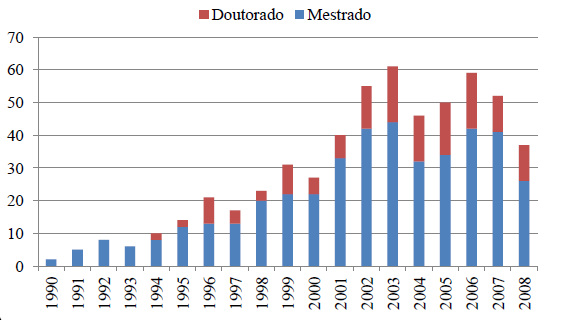
\includegraphics[scale=0.5]{figuras/figura-3}}
% 	}{
% 	\Fonte{os autores}
% }
% \end{figure}

% Ou então figuras podem ser incorporadas de arquivos externos, como é o caso da \autoref{fig-grafico-1}. Se a figura que ser incluída se tratar de um diagrama, um gráfico ou uma ilustração que você mesmo produza, priorize o uso de imagens vetoriais no formato PDF. Com isso, o tamanho do arquivo final do trabalho será menor, e as imagens terão uma apresentação melhor, principalmente quando impressas, uma vez que imagens vetorias são perfeitamente escaláveis para qualquer dimensão. Nesse caso, se for utilizar o Microsoft Excel para produzir gráficos, ou o Microsoft Word para produzir ilustrações, exporte-os como PDF e os incorpore ao documento conforme o exemplo abaixo. No entanto, para manter a coerência no uso de software livre (já que você está usando LaTeX e abnTeX),  teste a ferramenta InkScape\index{InkScape}. ao CorelDraw\index{CorelDraw} ou ao Adobe Illustrator\index{Adobe! Illustrator}.  De todo modo, caso não seja possível  utilizar arquivos de imagens como PDF, utilize qualquer outro formato, como JPEG, GIF, BMP, etc.  Nesse caso, você pode tentar aprimorar as imagens incorporadas com o software livre \index{Gimp}Gimp. Ele é uma alternativa livre ao Adobe Photoshop\index{Adobe! Photoshop}.

% \section{Usando Fórmulas Matemáticas}

% \lipsum[2]

% 	\begin{equation}
% 		\begin{aligned}
% 			x = a_0 + \cfrac{1}{a_1
% 				+ \cfrac{1}{a_2
% 					+ \cfrac{1}{a_3 + \cfrac{1}{a_4} } } }
% 		\end{aligned}
% 	\end{equation}

% \lipsum[3]

% 	\begin{equation}
% 		\begin{aligned}
% 			k_{n+1} = n^2 + k_n^2 - k_{n-1}
% 		\end{aligned}
% 	\end{equation}

% \lipsum[4]

% 	\begin{equation}
% 		\begin{aligned}
% 			\cos (2\theta) = \cos^2 \theta - \sin^2 \theta
% 		\end{aligned}
% 	\end{equation}
	
% \lipsum[5]

% 	\begin{equation}
% 		\begin{aligned}
% 			A_{m,n} =
% 			\begin{pmatrix}
% 			a_{1,1} & a_{1,2} & \cdots & a_{1,n} \\
% 			a_{2,1} & a_{2,2} & \cdots & a_{2,n} \\
% 			\vdots  & \vdots  & \ddots & \vdots  \\
% 			a_{m,1} & a_{m,2} & \cdots & a_{m,n}
% 			\end{pmatrix}
% 		\end{aligned}
% 	\end{equation}

% \lipsum[6]

% 	\begin{equation}
% 		\begin{aligned}
% 			f(n) = \left\{ 
% 			\begin{array}{l l}
% 			n/2 & \quad \text{if $n$ is even}\\
% 			-(n+1)/2 & \quad \text{if $n$ is odd}
% 			\end{array} \right.
% 		\end{aligned}
% 	\end{equation}
	
% \lipsum[7]

% \section{Usando Algoritmos}

% \lipsum[8]

% \begin{algorithm}[h!]
% 	\SetSpacedAlgorithm
% 	\caption{\label{alg:algoritmo_de_colonica_de_formigas}Algoritmo de Otimização por Colônia de Formiga}
% 	\Entrada{Entrada do Algoritmo}
% 	\Saida{Saida do Algoritmo}
% 	\Inicio{
% 		Atribua os valores dos parâmetros\;
% 		Inicialize as trilhas de feromônios\;
% 		\Enqto{não atingir o critério de parada}{
% 			\Para{cada formiga}{
% 				Construa as Soluções\;
% 			}
% 			Aplique Busca Local (Opcional)\;
% 			Atualize o Feromônio\;
% 		}	
% 	}		
% \end{algorithm}

% \lipsum[9]

% \section{Usando Código-fonte}

% \lipsum[10]

% \lstinputlisting[language=C++,caption={Hello World em C++}]{figuras/main.cpp}

% \lipsum[11]

% \begin{lstlisting}[language=Java,caption={Hello World em Java}]
% public class HelloWorld {
% 	public static void main(String[] args) {
% 		System.out.println("Hello World!");
% 	}
% }
% \end{lstlisting}

% \lipsum[11]

% \section{Usando Teoremas, Proposições, etc}

% Lorem ipsum dolor sit amet, consectetur adipiscing elit. Nunc dictum sed tortor nec viverra. consectetur adipiscing elit. Nunc dictum sed tortor nec viverra.

% \begin{teo}[Pitágoras]
% 	Em todo triângulo retângulo o quadrado do comprimento da
% 	hipotenusa é igual a soma dos quadrados dos comprimentos dos catetos.
% \end{teo}


% Lorem ipsum dolor sit amet, consectetur adipiscing elit. Nunc dictum sed tortor nec viverra. consectetur adipiscing elit. Nunc dictum sed tortor nec viverra.

% \begin{teo}[Fermat]
% 	Não existem inteiros $n > 2$, e $x, y, z$ tais que $x^n + y^n = z$
% \end{teo}

% Lorem ipsum dolor sit amet, consectetur adipiscing elit. Nunc dictum sed tortor nec viverra. consectetur adipiscing elit. Nunc dictum sed tortor nec viverra.

% \begin{prop}
% 	Para demonstrar o Teorema de Pitágoras...
% \end{prop}

% Lorem ipsum dolor sit amet, consectetur adipiscing elit. Nunc dictum sed tortor nec viverra. consectetur adipiscing elit. Nunc dictum sed tortor nec viverra.

% \begin{exem}
% 	Este é um exemplo do uso do ambiente exe definido acima.
% \end{exem}

% Lorem ipsum dolor sit amet, consectetur adipiscing elit. Nunc dictum sed tortor nec viverra. consectetur adipiscing elit. Nunc dictum sed tortor nec viverra.

% \begin{xdefinicao}
% 	Definimos o produto de ...
% \end{xdefinicao}

% Lorem ipsum dolor sit amet, consectetur adipiscing elit. Nunc dictum sed tortor nec viverra. consectetur adipiscing elit. Nunc dictum sed tortor nec viverra.

% \section{Usando Questões}


% Lorem ipsum dolor sit amet, consectetur adipiscing elit. Nunc dictum sed tortor nec viverra. consectetur adipiscing elit. Nunc dictum sed tortor nec viverra.

% \begin{questao}
% 	\item Esta é a primeira questão com alguns itens:
% 		\begin{enumerate}
% 			\item Este é o primeiro item
% 			\item Segundo item
% 		\end{enumerate}
% 	\item Esta é a segunda questão:
% 		\begin{enumerate}
% 			\item Este é o primeiro item
% 			\item Segundo item
% 		\end{enumerate}
% 	\item Lorem ipsum dolor sit amet, consectetur adipiscing elit. Nunc dictum sed tortor nec viverra. consectetur adipiscing elit. Nunc dictum sed tortor nec viverra.
% 		\begin{enumerate}
% 			\item consectetur
% 			\item adipiscing
% 			\item Nunc
% 			\item dictum
% 		\end{enumerate}
% \end{questao}

% \section{Citações}

% \subsection{Documentos com três autores}

% Quando houver três autores na citação, apresentam se os três, separados por ponto e vírgula, caso estes estejam após o texto. Se os autores estiverem incluídos no texto, devem ser separados por vírgula e pela conjunção "e".

% \citeautoronline{tresautores}

% \cite{tresautores}

% \subsection{Documentos com mais de três autores}
% Havendo mais de três autores, indica-se o primeiro seguido da expressão \textit{et al.} (do latim \textit{et alli}, que significa e outros), do ano e da página.

% \citeautoronline{quatroautores}

% \cite{quatroautores}

% \subsection{Documentos de vários autores}

% Havendo    citações    indiretas de    diversos    documentos    de    vários    autores, mencionados  simultaneamente e  que  expressam  a  mesma  ideia,  separam-se  os  autores  por ponto e vírgula, em ordem alfabética.

% \cite{tresautores, quatroautores}

% \section{Notas de Rodap\'{e}}

% Deve-se utilizar o sistema autor-data para as  citações no texto e o numérico para notas explicativas\footnote{Veja - se como exemplo desse tipo de abordagem o estudo de Netzer (1976)}. As notas de rodapé podem e devem ser alinhadas, a partir da segunda linha da mesma nota, abaixo da primeira letra da primeira palavra, de forma a destacar o expoente \footnote{Encontramos  esse  tipo  de  perspectiva  na  2ª  parte  do  verbete  referido  na  nota  anterior,  em  grande  parte  do estudo de Rahner (1962).} e sem espaço entre elas e com fonte menor (tamanho 10).

